\documentclass[11pt,a4paper]{article}

\usepackage[margin=1in]{geometry}
\usepackage[T1]{fontenc}
\usepackage[utf8]{inputenc}
\usepackage{lmodern}
\usepackage{microtype}
\usepackage{amsmath,amssymb}
\usepackage{booktabs}
\usepackage{graphicx}
\usepackage{caption}
\usepackage{subcaption}
\usepackage{float}
\usepackage[numbers,sort&compress]{natbib}
\usepackage[
  colorlinks=true,
  linkcolor=black,
  citecolor=black,
  urlcolor=blue
]{hyperref}

\bibliographystyle{plainnat}
\setlength{\parindent}{0pt}
\setlength{\parskip}{5pt}
\captionsetup{font=small,labelfont=bf}

\title{Cross-Sectional Return Prediction in a Small, Illiquid Equity Market:\\
Machine Learning Evidence from the Nairobi Securities Exchange}
\author{Felix Nyabuto}
\date{Preprint draft generated from reproducible research artifacts}

\begin{document}
\maketitle

\begin{abstract}
This paper asks whether machine-learning models can extract persistent
cross-sectional return-ranking information from a small, illiquid emerging
equity market, and whether that statistical predictability survives the
trading frictions of that market.  Using a 12-security Nairobi Securities
Exchange universe, walk-forward validation over 2024 provides evidence of
positive cross-sectional ranking information.  Random Forest is the strongest
tested estimator, with mean daily Spearman Information Coefficient (IC) of
0.133 and positive monthly IC in 12 of 12 months; the originally selected
LightGBM model achieves mean daily IC of 0.085 in the model-comparison
experiment.  Feature-group experiments show that simple returns and price
information contain much of the useful signal: a returns/price-only ablation
achieves mean daily IC of 0.125, compared with 0.111 for the full feature set
under the ablation protocol.  LLM-derived event variables contribute no
measured incremental IC in the evaluated historical window.  A retrospective
extended out-of-sample evaluation over 2025--2026 remains positive, with mean
daily IC of 0.0815 and positive monthly IC in 11 of 15 months, but is not a
pristine live holdout.  Economically, the evidence is much weaker: an
overlapping three-day Top-1 portfolio loses approximately 94.2\% cumulatively
under a 400 basis point round-trip cost assumption.  The main finding is
therefore a gap between statistical predictability and implementable
profitability in a high-friction market.
\end{abstract}

\section{Introduction}

Cross-sectional return prediction is usually studied in large, liquid markets
where extensive histories, broad security universes, and low trading costs make
statistical signals easier to diversify and monetize.  Small emerging markets
pose a different problem.  They may contain slow-moving information and
persistent frictions, but they also offer few securities, intermittent trading,
wide effective spreads, limited index data, and high explicit transaction
costs.  In such markets, evidence of return predictability is not equivalent
to evidence of an implementable trading strategy.

This paper studies that distinction using equities listed on the Nairobi
Securities Exchange (NSE).  The empirical question is: can machine-learning
models extract persistent cross-sectional return-ranking information from a
small, illiquid emerging equity market, and does that statistical
predictability survive the trading frictions of that market?  The answer is
qualified.  Within the studied 12-security universe, the experiments provide
evidence of positive out-of-sample ranking information.  However, the tested
portfolio rules do not establish economic profitability once realistic
round-trip costs are imposed.

The paper makes five contributions.  First, it provides evidence of persistent
cross-sectional ranking information in a small African equity universe.
Second, it shows that much of the predictive information is contained in
simple price and return variables rather than in richer feature groups.  Third,
it documents that estimator choice matters: Random Forest outperforms the
originally selected LightGBM model in the 2024 comparison.  Fourth, it shows
that measurable ranking predictability need not survive trading frictions.
Fifth, it provides a reproducible evaluation framework combining walk-forward
validation, dependence-aware inference, feature ablations, retrospective
extended out-of-sample evaluation, survivorship auditing, permutation
importance, and explicit cost-sensitive portfolio simulation.

The remainder of the paper proceeds as follows.  Section~\ref{sec:literature}
reviews related work.  Section~\ref{sec:data} describes the market and data.
Section~\ref{sec:method} presents the prediction and evaluation methodology.
Sections~\ref{sec:results}--\ref{sec:economic} report ranking, feature, and
economic results.  Section~\ref{sec:robustness} summarizes robustness tests,
Section~\ref{sec:limitations} discusses limitations, and
Section~\ref{sec:conclusion} concludes.

\section{Related Literature}
\label{sec:literature}

The study is related to empirical asset pricing and machine learning.
\citet{fama1992cross} and a large subsequent literature frame the
cross-section of returns as an empirical object explained by security
characteristics.  \citet{gu2020empirical} show that machine-learning methods
can improve expected-return measurement in broad U.S. equity data, especially
when nonlinear interactions among characteristics matter.  The present paper
uses a much smaller and less liquid setting, where the relevant question is
not whether a high-dimensional model can improve a large-universe factor
portfolio, but whether any rank information survives the sample-size and
trading-friction constraints of a small exchange.

The model set includes Random Forests \citep{breiman2001random} and LightGBM
\citep{ke2017lightgbm}.  Both are tree-based estimators, but the empirical
results below show that the choice between them matters.  The paper is also
connected to momentum and reversal evidence, beginning with
\citet{jegadeesh1993returns}; in the NSE data, simple return and price
features are central to the observed predictability.

Illiquidity is central to interpretation.  \citet{amihud2002illiquidity}
links illiquidity to expected returns, while \citet{lesmond1999transaction}
emphasize the importance of transaction-cost measurement.  Emerging equity
markets also differ in volatility, integration, and liquidity structure
\citep{bekaert1997emerging}.  These considerations motivate the separation
between statistical ranking quality and economic profitability.

The inference design responds to known risks in return-predictability
research.  Overlapping labels and serial dependence motivate HAC/Newey--West
standard errors \citep{newey1987simple}.  Multiple-testing and data-mining
concerns in the cross-section of expected returns motivate restrained claims
and robustness checks \citep{harvey2016cross}.  Finally, although recent work
studies LLMs as financial text processors or predictors
\citep{lopezlira2023chatgpt}, the experiments here do not find an incremental
LLM contribution in the evaluated historical window.

\section{Market and Data}
\label{sec:data}

The NSE is a small, relatively illiquid equity market.  The studied universe
contains 12 securities: ABSA, BAMB, BAT, BRIT, COOP, EABL, EQTY, JUB, KCB,
NMG, SCBK, and SCOM.  The main reproduction snapshot spans 2019-01-02 to
2024-12-31 and contains 18,240 security-day rows.  The 2024 retrospective
out-of-sample evaluation contains 3,048 security-day observations over 254
trading days.

\begin{table}[t]
\centering
\caption{Dataset and evaluation summary.}
\label{tab:dataset}
\small
\begin{tabular}{@{}lr@{}}
\toprule
Quantity & Value \\
\midrule
Securities & 12 \\
2019--2024 rows & 18,240 \\
2019--2024 dates & 2019-01-02 to 2024-12-31 \\
2024 test security-days & 3,048 \\
2024 test trading days & 254 \\
2025--2026 extended rows & 3,840 \\
2025--2026 extended trading days & 319 \\
Primary target & \texttt{label\_3d\_net\_alpha} \\
\bottomrule
\end{tabular}
\end{table}


Feature groups include return and price variables, momentum/reversal
variables, liquidity and volume proxies, NSE microstructure variables,
macroeconomic and exchange-rate variables, and LLM/event variables.  The
primary implementation target is \texttt{label\_3d\_net\_alpha}, a three-day
forward net-return label after the configured cost assumption.  Because
historical benchmark data are incomplete, the label should not be interpreted
as clean market-model alpha in all periods.

Universe construction is an important limitation.  The snapshot is a balanced
12-security seed universe, not a reconstructed historical universe of all NSE
listings.  Delisted, failed, or historically illiquid securities are absent.
Consequently, claims are restricted to the studied universe.

\section{Methodology}
\label{sec:method}

The predictive task is cross-sectional ranking.  For each trading day, models
score available securities, and evaluation compares the rank ordering of
scores with realized three-day forward net returns.  The primary rank metric
is the daily cross-sectional Spearman Information Coefficient (IC).  Monthly
IC values are averages of daily cross-sectional ICs within each calendar
month.

Model fitting uses temporal walk-forward validation.  For each test month, the
training data end before the validation and test windows, and no future test
observations are used in fitting.  The main 2024 comparison evaluates Random
Forest, LightGBM, linear and Ridge regressions, simple reversal and momentum
rules, and random rankings.  Statistical inference for the daily IC series
uses HAC/Newey--West standard errors with lag 3 to account for dependence from
overlapping three-day labels.

Economic evaluation uses overlapping three-day sleeves.  Each signal date
forms a Top-\(k\) long-only sleeve using the highest-ranked securities.
Sleeves are converted to daily equivalent returns and averaged across active
sleeves.  The simulation reports cumulative return, annualized volatility,
Sharpe ratio, maximum drawdown, sleeve hit rate, and cost sensitivity across
round-trip cost assumptions.  This design is intentionally simple: it tests
whether ranking quality survives a transparent implementation rule before
adding portfolio optimization complexity.

\section{Empirical Results}
\label{sec:results}

\subsection{2024 Walk-Forward Ranking Performance}

The 2024 LightGBM reproduction gives positive monthly test IC in 11 of 12
months and mean monthly test IC of 0.085.  This is evidence of ranking
information, but not evidence that LightGBM is the best available estimator.
Figure~\ref{fig:monthly_ic} shows monthly IC for selected models.

\begin{figure}[t]
\centering
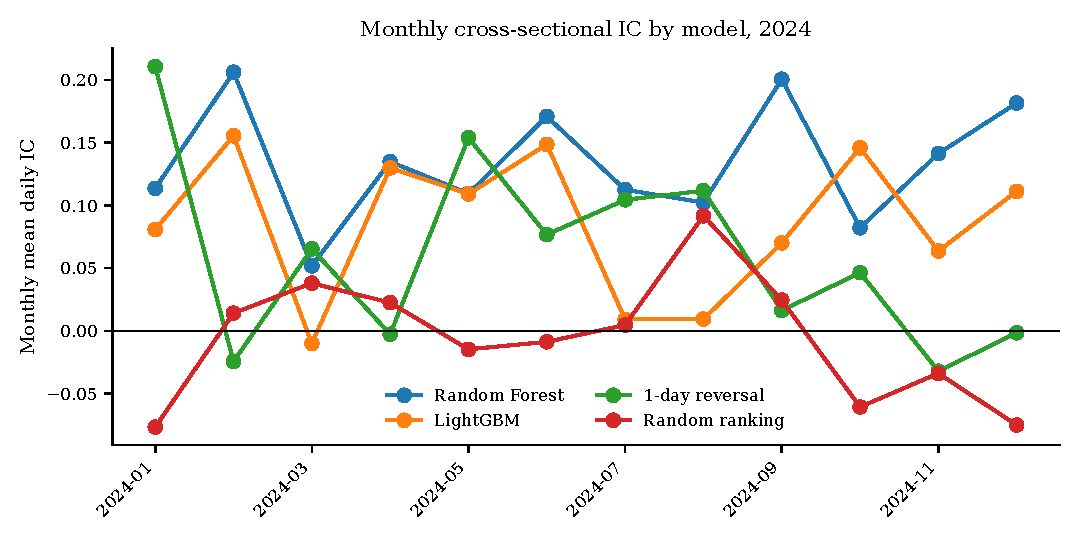
\includegraphics[width=0.92\textwidth]{figures/fig1_monthly_ic_by_model.pdf}
\caption{Monthly cross-sectional IC by model.  Values are monthly averages of
daily cross-sectional Spearman ICs.}
\label{fig:monthly_ic}
\end{figure}

\subsection{Model Comparison}

Table~\ref{tab:model_comparison} reports the 2024 model comparison.  Random
Forest has the highest mean daily IC, 0.133, and positive IC in all 12 months.
LightGBM achieves mean daily IC of 0.085 and positive IC in 11 of 12 months.
Simple reversal rules are positive but weaker, while momentum rules are
negative in this horizon and sample.

\begin{table}[t]
\centering
\caption{Model comparison on the 2024 retrospective out-of-sample period.}
\label{tab:model_comparison}
\small
\begin{tabular}{@{}lrrrrr@{}}
\toprule
Model & Mean IC & Median IC & ICIR & Pos. months & Top-1 hit \\
\midrule
Random Forest & 0.133 & 0.155 & 0.411 & 12/12 & 16.1\% \\
LightGBM & 0.085 & 0.087 & 0.279 & 11/12 & 16.9\% \\
1-day reversal & 0.062 & 0.042 & 0.202 & 8/12 & 16.5\% \\
3-day reversal & 0.056 & 0.045 & 0.189 & 9/12 & 16.9\% \\
Ridge regression & 0.019 & 0.038 & 0.060 & 8/12 & 16.1\% \\
Linear regression & 0.019 & 0.038 & 0.060 & 8/12 & 16.1\% \\
Random ranking & -0.006 & 0.000 & -0.021 & 6/12 & 9.1\% \\
5-day momentum & -0.049 & -0.056 & -0.157 & 3/12 & 14.6\% \\
20-day momentum & -0.052 & -0.046 & -0.166 & 4/12 & 13.4\% \\
\bottomrule
\end{tabular}
\end{table}


\begin{figure}[t]
\centering
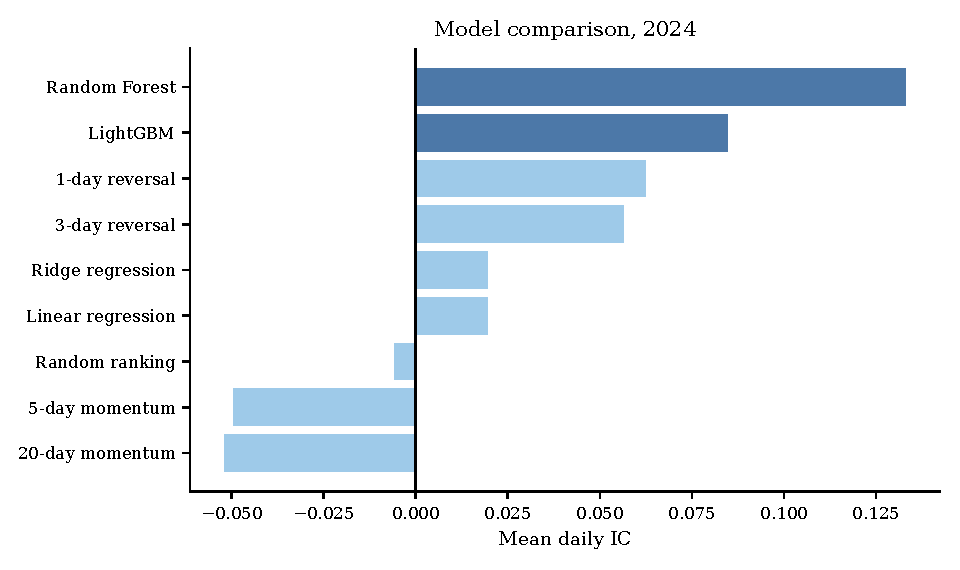
\includegraphics[width=0.82\textwidth]{figures/fig3_model_comparison.pdf}
\caption{Mean daily IC by model in the 2024 comparison.}
\label{fig:model_comparison}
\end{figure}

\subsection{Statistical Inference}

The LightGBM daily IC series is statistically positive in 2024 under
dependence-aware inference.  Table~\ref{tab:inference} reports the HAC
estimate.  The mean daily IC is 0.0846, with a 95\% confidence interval of
[0.0437, 0.1254] and p-value \(6.59\times 10^{-5}\).  This supports a claim
of ranking predictability for the evaluated period.  It does not establish
economic profitability.

\begin{table}[t]
\centering
\caption{Dependence-aware inference for the 2024 LightGBM daily IC series.}
\label{tab:inference}
\small
\begin{tabular}{@{}lr@{}}
\toprule
Statistic & Value \\
\midrule
Days & 254 \\
Mean daily IC & 0.0846 \\
Median daily IC & 0.0874 \\
IC standard deviation & 0.3027 \\
ICIR & 0.2794 \\
HAC lag & 3 \\
HAC standard error & 0.0208 \\
95\% CI & [0.0437, 0.1254] \\
t-statistic & 4.058 \\
p-value & 6.59e-05 \\
\bottomrule
\end{tabular}
\end{table}


\subsection{Extended 2025--2026 Retrospective OOS}

The extended evaluation covers 2025-01-02 to 2026-03-31.  It is best described
as retrospective extended out-of-sample evidence, not as a pristine live
holdout, because development history would be needed to prove that the period
was not inspected during model design.  The mean daily IC is 0.0815 and 11 of
15 months are positive.

\begin{table}[t]
\centering
\caption{Extended 2025--2026 retrospective out-of-sample evaluation.}
\label{tab:extended_oos}
\small
\begin{tabular}{@{}lr@{}}
\toprule
Statistic & Value \\
\midrule
Classification & Retrospective extended OOS \\
Period & 2025-01-02 to 2026-03-31 \\
Rows & 3,840 \\
Trading days & 319 \\
Mean daily IC & 0.081 \\
Median daily IC & 0.091 \\
Positive months & 11/15 \\
Top-1 hit rate & 14.4\% \\
\bottomrule
\end{tabular}
\end{table}


\begin{figure}[t]
\centering
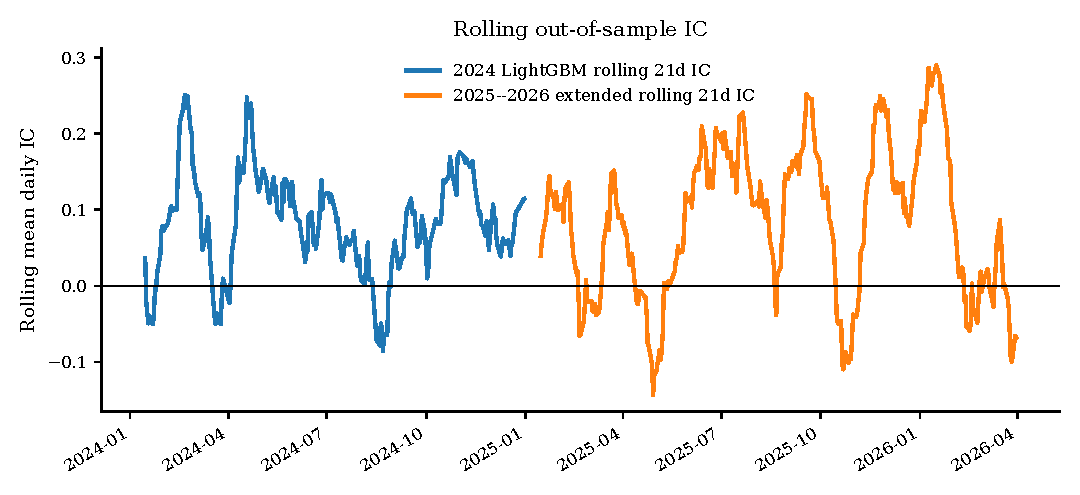
\includegraphics[width=0.92\textwidth]{figures/fig2_rolling_ic.pdf}
\caption{Rolling 21-day out-of-sample IC in the 2024 reproduction and the
2025--2026 retrospective extended evaluation.}
\label{fig:rolling_ic}
\end{figure}

\section{What Drives Predictability?}
\label{sec:drivers}

Feature-group ablations indicate that simple price and return variables
explain much of the predictive performance.  In the ablation experiment, the
returns/price-only feature set achieves mean daily IC of 0.125, while the full
feature set achieves 0.111.  This does not imply that additional feature
groups are useless in all settings, but it does mean that this experiment does
not support a claim that macroeconomic, microstructure, FX, event, or LLM
features improve prediction.

\begin{table}[t]
\centering
\caption{Feature-group ablations under the 2024 walk-forward protocol.}
\label{tab:ablations}
\small
\begin{tabular}{@{}lrrrrr@{}}
\toprule
Feature set & Mean IC & Median IC & Pos. months & Top-1 hit & Features \\
\midrule
Returns/price only & 0.125 & 0.119 & 12/12 & 22.0\% & 9 \\
Full feature set & 0.111 & 0.122 & 11/12 & 16.5\% & 62 \\
Momentum/reversal & 0.075 & 0.063 & 10/12 & 19.7\% & 8 \\
NSE microstructure & 0.034 & 0.040 & 9/12 & 13.0\% & 15 \\
Volume/liquidity & 0.002 & 0.000 & 5/12 & 9.4\% & 9 \\
Macro variables & -- & -- & -- & 6.3\% & 7 \\
KES/USD only & -- & -- & -- & 6.3\% & 2 \\
LLM/event variables & -- & -- & -- & 6.3\% & 10 \\
\bottomrule
\end{tabular}
\end{table}


\begin{figure}[t]
\centering
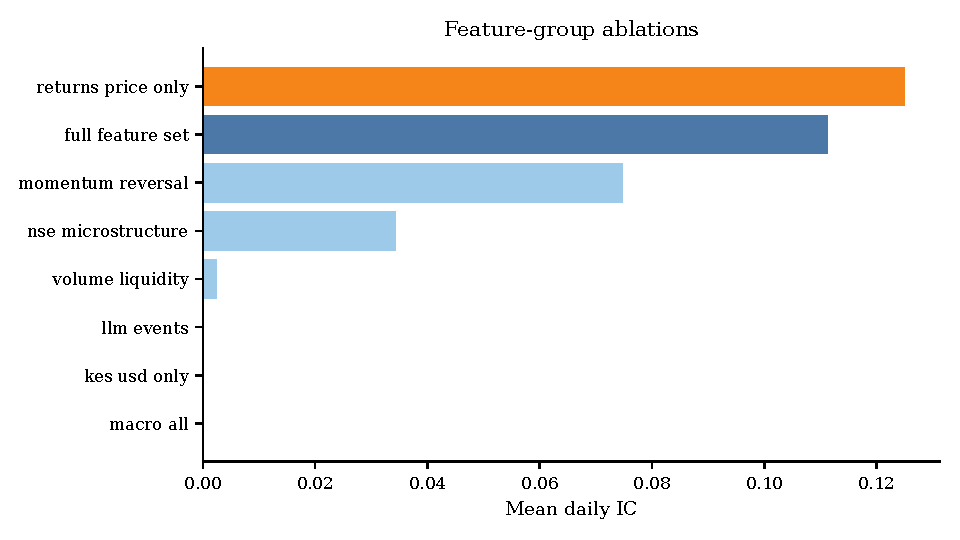
\includegraphics[width=0.82\textwidth]{figures/fig4_feature_ablations.pdf}
\caption{Feature-group ablation results.  The returns/price-only feature set
outperforms the full feature set in this experiment.}
\label{fig:ablations}
\end{figure}

Permutation importance is consistent with the ablation evidence.
Figure~\ref{fig:permutation} shows that permuting returns/price variables and
momentum/reversal variables produces the largest IC drops among interpretable
feature groups.  LLM/event variables have zero measured IC drop in the
historical window.  These results should not be read causally: correlated
features and small samples can distort both ablation and permutation
importance.

\begin{figure}[t]
\centering
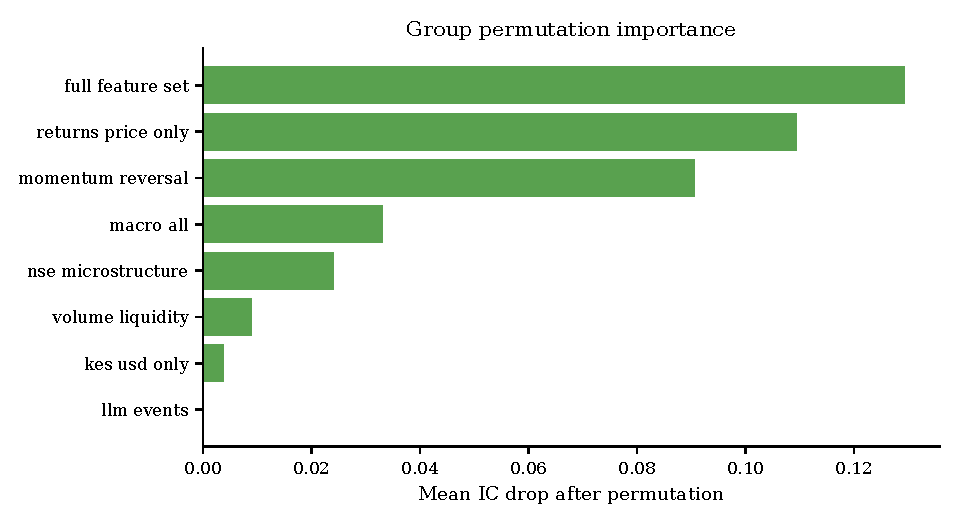
\includegraphics[width=0.82\textwidth]{figures/fig5_permutation_importance.pdf}
\caption{Group permutation importance.  Importance is measured as the drop in
mean daily IC after permuting each feature group in the test set.}
\label{fig:permutation}
\end{figure}

\section{Economic Evaluation}
\label{sec:economic}

The portfolio tests show a sharp gap between ranking predictability and
economic implementation.  Table~\ref{tab:portfolio} reports cost sensitivity
for overlapping three-day Top-\(k\) sleeves.  The most important result is the
Top-1 portfolio at 400 bps round-trip costs: it loses approximately 94.2\%
cumulatively in 2024, with maximum drawdown of approximately 94.2\%.  This
result rules out a claim of demonstrated profitability under the tested
trading assumptions.

\begin{table}[t]
\centering
\caption{Portfolio and transaction-cost sensitivity for overlapping three-day sleeves.}
\label{tab:portfolio}
\small
\begin{tabular}{@{}lrrrrrr@{}}
\toprule
Rule & Cost bps & Total ret. & Sharpe & Max DD & Sleeve hit & Mean sleeve ret. \\
\midrule
Top-1 & 0 & 80.8\% & 6.29 & -9.9\% & 57.1\% & 0.78\% \\
Top-1 & 100 & -22.4\% & -1.73 & -30.0\% & 43.3\% & -0.22\% \\
Top-1 & 400 & -94.2\% & -7.20 & -94.2\% & 16.9\% & -3.22\% \\
Top-1 & 600 & -99.0\% & -7.47 & -99.0\% & 8.3\% & -5.22\% \\
Top-2 & 0 & 48.1\% & 5.06 & -5.9\% & 60.2\% & 0.51\% \\
Top-2 & 100 & -36.5\% & -3.83 & -40.0\% & 40.2\% & -0.49\% \\
Top-2 & 400 & -95.3\% & -9.83 & -95.3\% & 8.3\% & -3.49\% \\
Top-2 & 600 & -99.2\% & -10.11 & -99.2\% & 2.8\% & -5.49\% \\
Top-3 & 0 & 74.3\% & 8.23 & -4.5\% & 61.0\% & 0.69\% \\
Top-3 & 100 & -25.2\% & -2.78 & -32.3\% & 39.4\% & -0.31\% \\
Top-3 & 400 & -94.4\% & -10.27 & -94.3\% & 6.7\% & -3.31\% \\
Top-3 & 600 & -99.0\% & -10.64 & -99.0\% & 3.5\% & -5.31\% \\
\bottomrule
\end{tabular}
\end{table}


\begin{figure}[t]
\centering
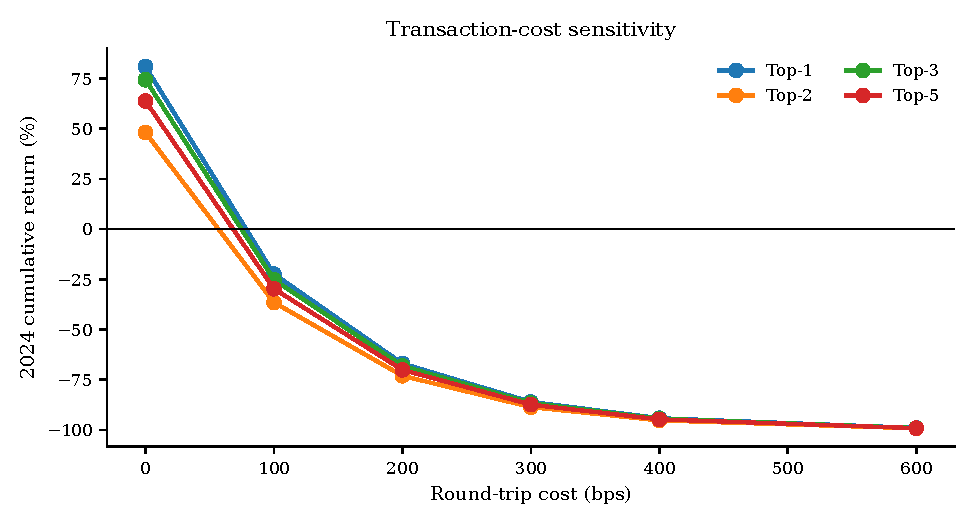
\includegraphics[width=0.86\textwidth]{figures/fig6_cost_sensitivity.pdf}
\caption{Transaction-cost sensitivity for Top-\(k\) overlapping sleeves.  The
poor 400 bps performance is not hidden by axis truncation.}
\label{fig:cost_sensitivity}
\end{figure}

\begin{figure}[t]
\centering
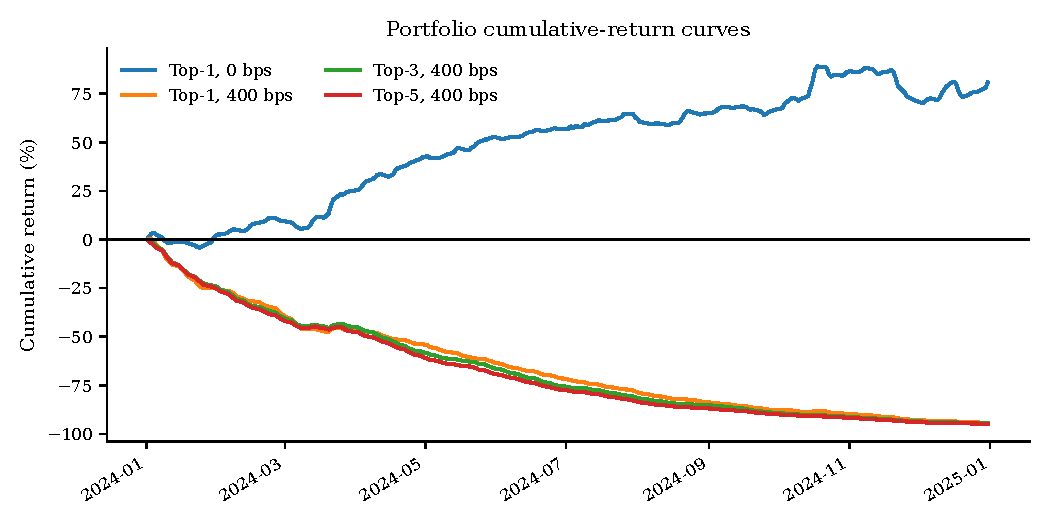
\includegraphics[width=0.92\textwidth]{figures/fig7_cumulative_returns.pdf}
\caption{Portfolio cumulative-return curves.  The Top-1, 400 bps curve
illustrates the economic failure of a naive implementation despite positive
ranking IC.}
\label{fig:cumulative}
\end{figure}

\begin{figure}[t]
\centering
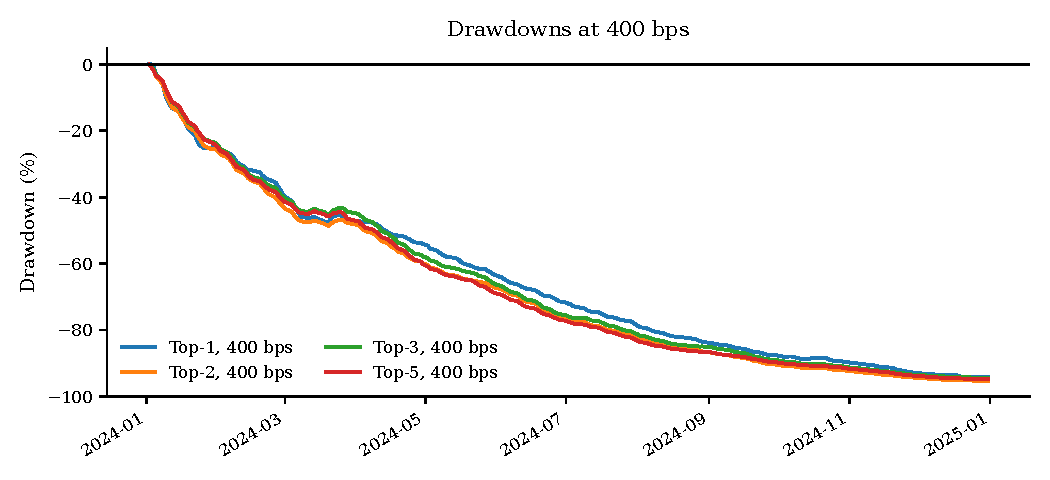
\includegraphics[width=0.92\textwidth]{figures/fig8_drawdowns.pdf}
\caption{Drawdown curves at 400 bps round-trip costs.}
\label{fig:drawdowns}
\end{figure}

\section{Robustness}
\label{sec:robustness}

The completed robustness experiments support the broad existence of ranking
information while weakening model-specific claims.  Random Forest has mean
daily IC of 0.133, positive monthly IC in 12 of 12 months, and outperforms
LightGBM in the 2024 comparison.  LightGBM results are broadly stable across
random seeds in the full-feature ablation protocol, with mean daily IC near
0.109--0.113.  A rolling three-year LightGBM window remains positive but
weaker, with mean daily IC of 0.083 and positive IC in 9 of 12 months.  The
one-day and five-day label robustness tests also remain positive, though they
answer different economic questions from the primary three-day target.

These checks do not eliminate all concerns.  The sample is small, the universe
is selected, and the economic tests remain highly sensitive to transaction
costs.  Robustness here should therefore be understood as evidence that the
ranking result is not a one-off artifact of a single LightGBM seed, not as
proof of an implementable strategy.

\section{Limitations}
\label{sec:limitations}

Several limitations constrain interpretation.  First, the cross-section
contains only 12 securities.  Security-day row counts therefore overstate the
effective sample size because returns share market and macro shocks and
labels overlap across dates.  Second, the universe is a 12-name seed universe,
not a reconstructed historical NSE universe.  Survivorship and
universe-selection risk remain unresolved.  Third, the 2025--2026 experiment
is retrospective extended out-of-sample evidence rather than a pristine live
holdout.  Fourth, transaction costs are estimated rather than observed from
order-level execution records.  Fifth, full historical index, order-book, and
bid--ask data are incomplete, limiting both alpha construction and cost
measurement.  Sixth, feature-importance results are descriptive rather than
causal.  Finally, LLM/event variables are not validated as predictive
contributors in the historical sample.

\section{Conclusion}
\label{sec:conclusion}

The experiments provide evidence that machine-learning models can extract
cross-sectional ranking information from the studied NSE universe.  The
evidence is strongest for Random Forest in 2024, and the extended 2025--2026
retrospective evaluation remains positive.  However, the source of
predictability appears simple: returns and price variables explain much of the
performance, while richer macro, microstructure, FX, event, and LLM feature
groups do not show demonstrated incremental value in the completed
experiments.

The economic conclusion is more severe.  Under the tested overlapping-sleeve
implementation, a Top-1 strategy at 400 bps round-trip costs loses
approximately 94.2\% cumulatively.  The central contribution of the paper is
therefore not a profitable trading rule.  It is evidence that statistical
predictability, ranking quality, economic significance, and implementable
profitability are distinct concepts in a high-friction emerging market.  In
the studied NSE universe, the first two are supported; the last is not.

\appendix

\section{Appendix: Full Monthly LightGBM Results}

The reproduced 2024 LightGBM monthly test ICs are 0.081, 0.155, -0.010,
0.130, 0.109, 0.149, 0.009, 0.009, 0.070, 0.146, 0.064, and 0.111.  The mean
monthly test IC is 0.085 and 11 of 12 months are positive.

\section{Appendix: Implementation Traceability}

All main tables and figures are generated by the asset-generation script in
the publication directory.  The script reads the reproduction, baseline,
daily-IC, and phases 9--15 output folders; it then writes LaTeX tables and
vector PDF figures into the publication tree.  The manuscript consumes only
those generated tables and figures.

\bibliography{references}

\end{document}
